\chapter{Esempio: divisore di tensione}

\begin{figure}
 \centering
 \subfloat[Divisore di tensione]{\label{fig:resol}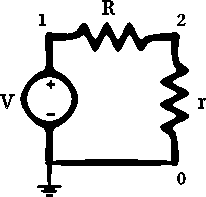
\includegraphics[scale=0.90]{immagini/resol.pdf}}\hspace{50pt}
 \subfloat[Modello dipendente]{\label{fig:resoldip}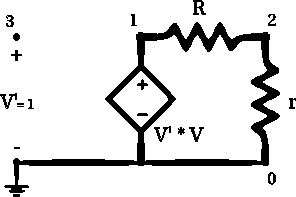
\includegraphics[scale=0.90]{immagini/resoldip.pdf}}\\\vspace{20pt}
 \subfloat[Modello equivalente]{\label{fig:resoleq}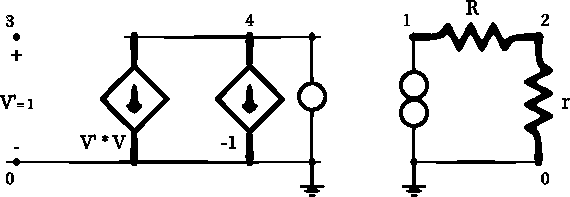
\includegraphics[scale=0.90]{immagini/resoleq.pdf}}\\\vspace{20pt}
 \subfloat[Circuito modificato]{\label{fig:resolmod}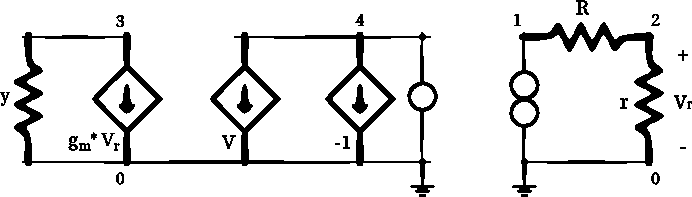
\includegraphics[scale=0.90]{immagini/resolmod.pdf}}\\\vspace{20pt}
 \subfloat[Grafi in corrente (G.I.) e in tensione (G.V.)]{\label{fig:resolgs}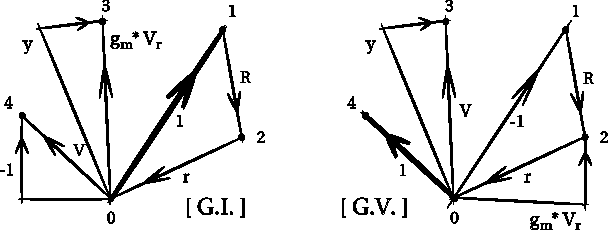
\includegraphics{immagini/resolgs.pdf}}
 \caption{Analisi successiva per il divisore di tensione}
 \label{fig:resolall}
\end{figure}

Per terminare questa parte, sfruttando la teoria esposta fino ad ora, viene proposto un esempio di analisi simbolica, dal disegno fino alle fasi di risoluzione per un semplice circuito. Dall'esempio si potrà osservare come anche una rete elementare finisca col trasformarsi, attraverso mutazioni e adattamenti successivi, in una struttura equivalente ben più complessa ma risolvibile. Non deve spaventare il fatto che un semplice circuito composto da tre componenti si traduca, alla fine, in una rete contenente tre resistenze, tre generatori controllati e un nullore (cioè una coppia nullatore-noratore), poiché questo altro non è che l'inevitabile risultato dell'applicazione delle tecniche precedentemente esposte.

Le varie fasi attraversate sono riportate in successione in figura \ref{fig:resolall}. Nella \ref{fig:resol} si ha il circuito che si vuole analizzare, un semplice divisore di tensione composto di un generatore di tensione e due resistenze; un totale di tre nodi è richiesto dall'utente per il disegno, è noto però che questa quantità lieviterà a causa della richiesta di nodi fittizi messa in atto da specifici componenti.

In figura \ref{fig:resoldip} si opera la prima modifica, ovvero si attua la sostituzione del generatore di tensione rendendo di fatto quello presente nel circuito sottomesso un generatore di tensione controllato in tensione. Questo è possibile per il fatto che durante le fasi di risoluzione si considera come generatore unico interno al circuito un componente fittizio ininfluente da cui tutti gli altri dipenderanno (ovvero, i generatori di corrente e di tensione diventeranno a loro volta generatori controllati in tensione dall'elemento fittizio). Col termine ininfluente si indica il fatto che esso è trattato come elemento non simbolico e ha valore unitario, per cui sistemando in modo corretto i parametri coinvolti non influisce affatto sul risultato finale. Dall'immagine si può notare come, appunto, la tensione ottenuta attraverso il generatore controllato abbia di fatto valore identico a quella proposta nel circuito originale.

In figura \ref{fig:resoleq} viene fatto un ulteriore passo avanti, avviene cioè la sostituzione del generatore controllato precedentemente inserito col suo modello equivalente, composto da generatori di corrente controllati in tensione e nullori. Se già al passo precedente il numero di nodi richiesti era aumentato, un'ulteriore crescita si ha in questa sede, portando il totale a cinque nodi e ritrovandosi con un circuito ben lungi dall'assomigliare all'originale proposto. Ancora, sebbene possano risultare difficilmente comprensibili i valori associati ai diversi elementi coinvolti durante la sostituzione, rifacendosi ai capitoli precedenti si ha che vale per il generatore di tensione controllato in tensione, dal modello equivalente (dove $g$ e $g'$ siano i parametri dei generatori di corrente controllati in tensione):
$$ V_{out} = -\frac{g}{g'}\ast V_{in};\quad I_ {in} = 0; $$
Per cui per $V_{in}$ unitario, posto $g'$ pari a $-1$, si può modellare $g$ a piacimento così da ottenere il valore desiderato per $V_{out}$. Nel caso specifico, $g$ ha assunto il valore associato al generatore indipendente presente nel circuito originale.

Procedendo, nella \ref{fig:resolmod} viene illustrato come risulta la rete una volta modificata, ovvero una volta aggiunta la circuiteria d'ingresso. Questa, ricordiamo, è utile allo scopo di rendere facilmente estrapolabile, dal computo finale dell'equazione, l'insieme di elementi che andranno a costituire numeratore e denominatore della funzione d'uscita. Il circuito finalmente modificato e rielaborato secondo le necessarie sostituzioni, si presenta nella sua forma finale e può essere sottoposto al risolutore vero e proprio che si aspetta, appunto, un particolare tipo di reti composte solo ed esclusivamente da specifici componenti (tutti quelli che è in grado realmente di trattare).

\paragraph{}

L'operazione successiva consiste nello spostarsi dallo spazio dei circuiti elettrici in quello dei grafi\graffito{Dovrebbe far riflettere l'idea che il problema attraversa orizzontalmente aree tematiche diverse, spogliandosi del suo significato originario e andando a trovare una soluzione concreta altrove, per poi adottarla nel contesto di partenza}, attraverso una traduzione componente per componente della rete finale ottenuta. In figura \ref{fig:resolgs} sono riportati i due grafi in tensione e in corrente ottenuti da questo processo, evidenziando in grassetto gli archi dovuti al nullore (che, sottolineiamo, devono essere forzati in ogni albero di copertura comune) e quello che si potrebbe definire il peso del singolo arco, ovvero il valore ad esso associato (in questo esempio si assume, senza perdita di generalità, un'analisi prettamente simbolica). Sui due grafi così ottenuti non resta che applicare l'algoritmo di ricerca degli alberi di copertura comuni, il quale restituirà i seguenti elenchi di archi (indicati col peso associato per essere distinti, laddove ve ne siano più d'uno fra una stessa coppia di nodi):
\begin{enumerate}
 \item $ \left[\; 1,\; y,\; -1,\; R\;\right] $
 \item $ \left[\; 1,\; y,\; -1,\; r\;\right] $
 \item $ \left[\; 1,\; g_m * V_r,\; V,\; R\;\right] $
\end{enumerate}
Ovviamente, avendo cinque nodi, gli alberi sono composti da quattro archi ognuno. Tralasciando il calcolo del parametro $\varepsilon_i$, il quale procedimento si descrive come la mera riduzione della matrice d'incidenza associata ai singoli alberi e quindi al calcolo del determinante di detta matrice, si nota fin da subito come da quanto ottenuto si possano ricavare immediatamente i dati necessari al calcolo dell'espressione finale. Seguendo infatti l'ordine degli alberi sopra riportati e considerando l'approccio di scelta delle ammettenze sull'albero e delle impedenze sul coalbero, oltre che rifacendosi al fatto illustrato per cui gli alberi comprendenti il ramo $y$ vanno al denominatore e gli alberi contenenti il ramo $g_m * V_r$ vanno al numeratore, abbiamo quanto segue:
\begin{enumerate}
 \item Nessuna ammettenza sull'albero, impedenza $r$ sul coalbero.
 \item Nessuna ammettenza sull'albero, impedenza $R$ sul coalbero.
 \item Ammettenza $V$ sull'albero (nota: $V$ è un valore dovuto alla presenza del generatore di corrente controllato in tensione, da cui il suo ruolo come ammettenza), impedenza $r$ sul coalbero.
\end{enumerate}
Bisogna fare una precisazione sui rami $y$ e $g_m$. Nella pratica, anche laddove essi rechino dati significativi, bisogna interpretarli solo ed esclusivamente come marcatori per quegli alberi che andranno a comporre l'equazione finale. Pertanto, nonostante almeno uno di essi potrebbe dare il suo apporto in questa fase, una volta individuati ed estratti gli alberi da essi indicati, sono di fatto esclusi da ogni fase successiva e con loro il carico informativo trasportato.

Arrivati a questo punto, poiché la regola impone che si moltiplichino componenti di uno stesso albero e si sommino elementi su alberi differenti, si ricava come atteso:
$$ \frac{V * r}{R + r} $$

\paragraph{}

Inutile dire che il procedimento sopra descritto in maniera esaustiva e particolareggiata può essere snellito e migliorato sotto diversi aspetti e, nella realtà, discosta abbastanza da quello illustrato pur rimanendo fedele ai principi e alle linee guida che hanno pilotato l'illustrazione. Di fatto, per esempio, l'introduzione di un generatore globale fittizio da cui tutti vengano a dipendere è una richiesta che si scontra con le necessità di ridurre i tempi di calcolo, pertanto si può usare il primo generatore incontrato durante la sintesi ponendolo come globale e facendo dipendere da esso tutti i successivi. Allo stesso modo sarà inutile sostituire sorgenti indipendenti con sorgenti controllate, quindi quest'ultime con modelli equivalenti, quando in un unico passo si può applicare la trasformazione diretta saltando la fase intermedia.

Queste sono soltanto alcune delle tante possibilità di ottimizzazione della procedura messe in atto durante lo sviluppo vero e proprio.
